\documentclass[10pt,a4paper]{article}
\usepackage[utf8]{inputenc}
\usepackage{amsmath}
\usepackage{amsfonts}
\usepackage{amssymb}
\usepackage{graphicx}
\usepackage{fourier}
\author{José Jácome}
\title{Capítulo VII}
\begin{document}
%\chapter{Capitulo VII}
\section{SERIES DE POTENCIAS, DE TAYLOR Y DE LAURENT}
\subsection{Series de Potencias}
Una serie de potencias en el plano complejo es de la forma siguiente:
\begin{equation}
\sum_{n = 0}^{\infty} c_n (z-z_0)^n = c_0 + c_1(z-z_0) + c_2 (z-z_0)^2 + ... +  c_n (z-z_0)^n + ...
\end{equation}
donde $c_n$ son constantes reales y complejos llamados coeficientes "$z_0$" es constante y se llama \textit{centro de la serie},"$z$" es la variable compleja. \\
Si $z_0 = 0$ , la serie (1) se reduce a la forma $\displaystyle{\sum_{n = 0}^{\infty} c_n z^n = c_0 + c_1 z + c_2 z^2 + ... + }$ , serie de potencias z.\\
\textbf{OBSERVACIÓN.-}
\begin{itemize}
\item Diremos que la serie $\displaystyle{\sum_{n = 0}^{\infty} c_n (z-z_0)^n}$ es absolutamente convergente, $\forall z \epsilon C$ tal que $ \parallel z - z_0 \parallel  < R$ y es divergente, $\forall \epsilon  C$ , tal que $\parallel z - z_0 \parallel > R$
\item Si $\exists R > 0$ , tal que $\displaystyle{\sum_{n = 0}^{\infty} c_n (z-z_0)^n}$ converge absolutamente en $\parallel z - z_0 \parallel < R$ y si $0 < \rho < R$ , la serie $\displaystyle{\sum_{n = 0}^{\infty} c_n (z-z_0)^n}$ converge uniformente en $\parallel z - z_0 \parallel < \rho$
\item La serie $\displaystyle{\sum_{n = 0}^{\infty} c_n (z-z_0)^n}$ converge absolutamente  $\forall z \epsilon C$ (en particular en $z = z_0$) tal que $\parallel z - z_0 \parallel < R $ y si $0 < \rho < R$, entonces la serie converge uniformentente, $\forall z \epsilon C$ tal que $0< \parallel z - z_0 \parallel < \rho$
\item Al número $R > 0$ se llama radio de convergencia de las serie $\displaystyle{\sum_{n = 0}^{\infty} c_n (z-z_0)^n}$
\item Para $z \epsilon C$, se tiene $\parallel z - z_0 \parallel < R$, que se denomina región de convergencia.
\begin{center}
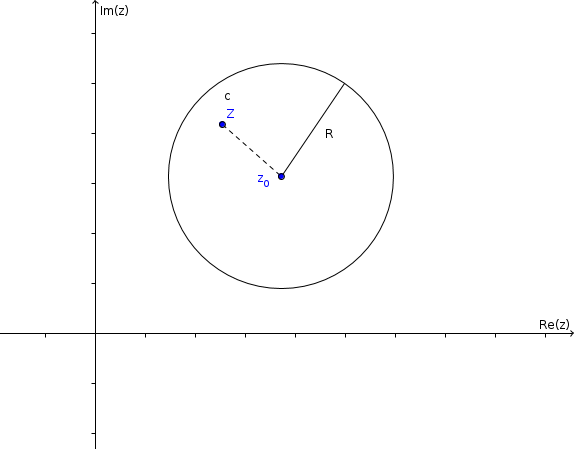
\includegraphics[scale=0.5]{1.png}
\end{center}
\item Para hallar el radio y región de convergencia de una serie de la forma $\displaystyle{\sum_{n = 0}^{\infty} c_n (z-z_0)^n}$, se utiliza el criterio de la razón, que esta caracterizada por el siguiente teorema
\end{itemize}
\subsection{TEOREMA (CRITERIO DE LA RAZÓN).-}
Sea $\displaystyle{\sum_{n = 0}^{\infty} c_n (z-z_0)^n}$ una serie de potencia en $C$ y sea $u_n = c_n (z-z_0)^n$, tal que $\displaystyle{\lim_{n \to \infty} \parallel \dfrac{u_{n+1}}{u_n}  \parallel = L }$ , entonces:
\begin{itemize}
\item[i)] Si $L<1$, la serie $\displaystyle{\sum_{n = 0}^{\infty} c_n (z-z_0)^n}$ converge absolutamente.
\item[ii)] Si $L>1$, la serie $\displaystyle{\sum_{n = 0}^{\infty} c_n (z-z_0)^n}$ diverge.
\item[iii)] Si $L=1$, el criterio no decide.
\end{itemize}
\textbf{OBSERVACIONES}
\begin{itemize}
\item Sea $\displaystyle{\sum_{n=0}^{\infty}}$ una serie de potencia tal que: $\displaystyle{\lim_{n \to \infty} \sqrt[n]{\parallel c_n \parallel} = L}$, entonces:
\begin{itemize}
\item[i)] Si $L=0$, entonces ($R= \infty$); la serie es convergente en todo el plano complejo C
\item[ii)] Si $L>0$, entonces $\displaystyle{R = \dfrac{1}{L}}$
\item[iii)] Si $L= \infty$, entonces ($R = 0$) converge solamente en el origen.
\end{itemize}
\item Sea $\displaystyle{\sum_{n=0}^{\infty} c_n z^n}$ uan serie de potencia tal que: $\displaystyle{\lim_{n \to \infty} \parallel \dfrac{c_{n+1}}{c_n} \parallel = L}$, entonces: 
\begin{itemize}
\item[i)] Si $L=0$, entonces ($R= \infty$)
\item[ii)] Si $L>0$, entonces $\displaystyle{R = \dfrac{1}{L}}$
\item[iii)] Si $L= \infty$, entonces $R = 0$
\end{itemize}
\end{itemize}
\subsection{FUNCIONES REPRESENTADAS MEDIANTE SERIES DE POTENCIAS.-}
%PAG 328%
La serie de potencia  $\displaystyle{\sum_{n = 0}^{\infty} c_n (z-z_0)^n}$, con radio de convergencia $R>0$, define una función de $z$, es decir:  $\displaystyle{f(z) = \sum_{n = 0}^{\infty} c_n (z-z_0)^n}$, donde $\displaystyle{D_f = {z  \epsilon  C  /  \parallel z - z_0 \parallel < R}}$ es decir que el dominio de $f(z)$ es la región de convergencia de la serie, por ejemplo consideramos la serie $\displaystyle{\sum_{n = 0}^{\infty} z^n = 1 + z + z^2 + ... + z^n+...}$ convergente, $\displaystyle{\forall z \epsilon C}$ tal que $\parallel z \parallel < R$ \\
Donde $\displaystyle{R = \lim_{n \to \infty} \parallel \dfrac{c_n}{c_{n+1}} \parallel = \lim_{n \to \infty} \parallel \dfrac{1}{1} \parallel = 1 }$ es decir la serie $\displaystyle{\sum_{n = 0}^{\infty} z^n}$ es convergente $\forall z \epsilon C$ tal que $\parallel z \parallel < 1$
%Grafico%
\begin{center}
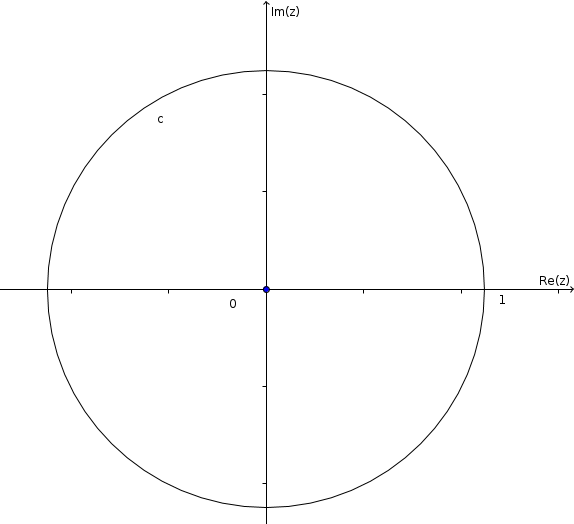
\includegraphics[scale=0.5]{2.png}
\end{center}
Luego la serie $\displaystyle{\sum_{n = 0}^{\infty} z^n}$ define la función $\displaystyle{\sum_{n = 0}^{\infty} z^n = \dfrac{1}{1-z}}$\\
\textbf{OBSERVACIÓN.-} Si $\displaystyle{f(z) = \sum_{n = 0}^{\infty} c_n (z-z_0)^n}$, entonces se dice que $f(z)$ es representada mediante la serie de potencia o se dice que $f(z)$ esta desarrolado mediante una serie de potencia.
\subsection{DERIVACIÓN E INTEGRACIÓN DE SERIES.-}
Sea $\displaystyle{f(z) = \sum_{n = 0}^{\infty} c_n (z-z_0)^n}$ una serie de potencia convergente $\forall z \epsilon C$ tal que $\displaystyle{\parallel z - z_0 \parallel < R}$ , $R > 0$ entonces:
$\displaystyle{f'(z) = \sum_{n = 0}^{\infty} n c_n (z-z_0)^{n-1}}$, convergente $\displaystyle{\forall z \epsilon C}$, tal que $\displaystyle{\parallel z - z_0 \parallel < R'}$ donde $\displaystyle{R = lim_{n \to \infty} \parallel \dfrac{c_n}{c_{n+1}} \parallel}$, entonces se tiene: \\
$\displaystyle{R' = \lim_{n \to \infty} \parallel \dfrac{n c_n}{(n+1) c_{n+1}} \parallel =\lim_{n \to \infty}  \dfrac{n}{n+1}  . \lim_{n \to \infty} \parallel \dfrac{c_n}{c_{n+1}} \parallel = 1  . \lim_{n \to \infty} \parallel \dfrac{c_n}{c_{n+1}} \parallel = \lim_{n \to \infty} \parallel \dfrac{c_n}{c_{n+1}} \parallel  = R}$ \\
por lo tanto $R = R'$\\
$\displaystyle{f''(z) = \sum_{n = 0}^{\infty} n (n-1) c_n (z-z_0)^{n-2}}$, converge $\forall z \epsilon C$, tal que $\displaystyle{\parallel z - z_0 \parallel < R''}$, de donde: \\
$\displaystyle{R'' = \lim_{n \to \infty} \parallel \dfrac{n (n-1) c_n}{n(n+1) c_{n+1}} \parallel =\lim_{n \to \infty}  \dfrac{n(n-1)}{n(n+1)}  . \lim_{n \to \infty} \parallel \dfrac{c_n}{c_{n+1}} \parallel = 1  . \lim_{n \to \infty} \parallel \dfrac{c_n}{c_{n+1}} \parallel = \lim_{n \to \infty} \parallel \dfrac{c_n}{c_{n+1}} \parallel  = R}$ \\ 
por lo tanto $R = R''$ \\
Las series obtenidas, derivando de la serie de potencia original tien el mismo radio de convergencia que la serie original. \\
Sea $\displaystyle{f(z) = \sum_{n = 0}^{\infty} c_n (z-z_0)^n}$ una serie de potencia convergente $\forall z \epsilon C$ tal que $\parallel z - z_0 \parallel < R$ \\
$\displaystyle{\int_{z_0}^{z} f(z) dz = \int_{z_0}^{z} \sum_{n = 0}^{\infty} c_n (z-z_0)^n dz = \sum_{n = 0}^{\infty} c_n \int_{z_0}^{z}  (z-z_0)^n dz =  \sum_{n = 0}^{\infty} \dfrac{c_n}{n+1} (z-z_0)^{n+1}}$, es convergente $\forall z \epsilon C$ tal que $\parallel z - z_0 \parallel < R$
\subsection{SERIE DE TAYLOR Y DE MACLAURIN COMPLEJA.-}
Sea  $\displaystyle{f(z) = \sum_{n = 0}^{\infty} c_n (z-z_0)^n}$ una serie de potencia convergente $\forall z \epsilon C$ tal que $\parallel z - z_0 \parallel < R$, calculando sus derivadas y evaluando en $z = z_0$ \\
$\displaystyle{f(z) = \sum_{n = 0}^{\infty} c_n (z-z_0)^n} \Rightarrow f(z_0) = c_0$ de donde $c_0 = f(z_0)$ \\
$\displaystyle{f'(z) = \sum_{n = 1}^{\infty} n c_n (z-z_0)^{n-1}} \Rightarrow f'(z_0) = c_1$ de donde $c_1 = f'(z_0)$ \\ 
$\displaystyle{f''(z) = \sum_{n = 2}^{\infty} n (n-1) c_n (z-z_0)^{n-2}} \Rightarrow f''(z_0) = 1.2.c_2$ de donde $c_2 = \dfrac{f''(z_0)}{2!}$ \\ 
$\displaystyle{f'''(z) = \sum_{n = 3}^{\infty} n (n-1)(n-2) c_n (z-z_0)^{n-3}} \Rightarrow f'''(z_0) = 1.2.3.c_3 = 3! c_3$ de donde $c_3 = \dfrac{f'''(z_0)}{3!}$ \\ 
.\\
.\\
.\\
%Revisar
$\displaystyle{f^{(m)}(z) = \sum_{n = m}^{\infty} n (n-1)(n-2)...2.1.c_n (z-z_0)^{n-m} = \sum_{n = m}^{\infty} n! c_n (z-z_0)^{n-m}}$ entonces  $f^(n) (z_0) = n! c_n$ de donde $c_n = \dfrac{f^{(n)} (z_0)}{n!}$ \\
como  $\displaystyle{f(z) = \sum_{n = 0}^{\infty} c_n (z-z_0)^n}$, desarrollando \\
$\displaystyle{f(z) = c_0 + c_1 (z-z_0) + c_2 (z-z_0)^2 + ... + c_n(z-z_0)^n+...}$\\
$\displaystyle{f(z) = f(z_0) +f'(z_0)(z-z_0) + \dfrac{f''(z_0)}{2!}(z-z_0)^2 + ... + \dfrac{f^{(n)}(z_0)}{n!}(z-z_0)^n+ ... }$\\

$\therefore$ \begin{equation}
f(z) = \sum_{n = 0}^{\infty} \dfrac{f^{(n)} (z_0)(z-z_0)^n}{n!}
\end{equation}
es la serie de Taylor alrededor de $z = z_0$\\
cuando $z_0 = 0$, se tiene la serie \begin{equation}
f(z) = \sum_{n = 0}^{\infty} \dfrac{f^{(n)}(0) z^n}{n!}
\end{equation}
que se denomina serie de MACLAURIN
\subsection{TEOREMA.-}
%PAg 331
Sea $f(z)$ una función analítica en $z_0$, entonces $f(z)$ tiene una representación en serie de Taylor $\displaystyle{f(z) = \sum_{n=0}^{\infty}\dfrac{f^{(n)}(z_0)(z-z_0)^n}{n!}}$, $\displaystyle{\forall z}$ en algún disco de centro en $z_0$\\
\begin{center}
 \bf \underline{Demostración}
 \end{center} 
 Como $f$ es analítica $\Rightarrow \exists$ un disco $\parallel z- z_0\parallel < r$ en donde $f$ es derivable, sea $\displaystyle{\gamma : \parallel z- z_0\parallel= \dfrac{r}{2}}$, entonces $f$ es derivable en todos los puntos sobre y dentro de $\gamma$.
 Sea $w \epsilon \gamma$ y $z$ cualquier punto dentro de $\gamma$, entonces escribiremos:\\
%Grafico pag 332 Revisar
\begin{center}
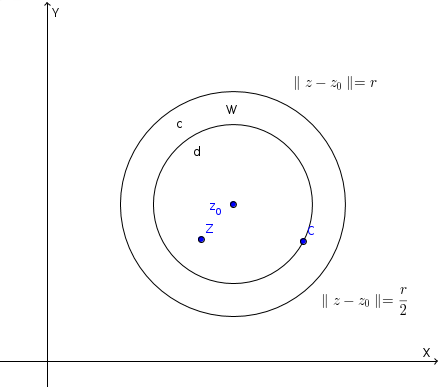
\includegraphics[scale=0.5]{3.png}
\end{center}
$\displaystyle{\dfrac{1}{w-z} = \dfrac{1}{w-z_0}. \dfrac{1}{1-\dfrac{z-z_0}{w-z_0}}}$ \textbf{... (1)}\\
como $w$ esta más lejos a $z_0$ que lo de z, entonces $\parallel  z - z_0\parallel < \parallel w - z_0 \parallel$ por lo tanto $\parallel \dfrac{z-z_0}{w-z_0} \parallel < 1$, mediante la serie geométrica se tiene:\\
\begin{center}
$\displaystyle{\dfrac{1}{1-\dfrac{z-z_0}{w-z_0}}= \sum_{n=0}^{\infty} (\dfrac{z - z_0}{w - z_0})^n}$ \textbf{... (2)}
\end{center}
reemplazando (2) en (1) se tiene: $\displaystyle{\dfrac{1}{w-z}= \dfrac{1}{w-z_0}\sum_{n=0}^{\infty} (\dfrac{z - z_0}{w - z_0})^n = \sum_{n=0}^{\infty} \dfrac{(z - z_0)^n}{(w - z_0)^{n+1}}}$ \\ ahora por la fórmula de la integral de Cauchy se tiene: \\
$\displaystyle{f(z) = \dfrac{1}{2 \pi i} \oint_\gamma \dfrac{f(w)}{w-z} dw = \dfrac{1}{2 \pi i} \oint_\gamma \dfrac{f(w)(z-z_0)^n}{(w-z)^{n+1}} dw }$\\
$\displaystyle{\sum_{n=0}^{\infty} [ \dfrac{1}{2 \pi i} \oint_\gamma \dfrac{f(w) dw}{(w-z_0)^{n+1}}] (z-z_0)^n}$ \textbf{... (3)}\\
pero se conoce que: $\displaystyle{\dfrac{1}{2 \pi i} \oint_\gamma \dfrac{f(w) dw}{(w-z_0)^{n+1}} = \dfrac{1}{n!} f^{(n)}(z_0)}$ \textbf{... (4)}\\
al reemplazar (4) con (3) se obtiene: $\displaystyle{f(z) = \sum_{n = 0}^{\infty} \dfrac{f^{(n)} (z_0)}{n!} (z-z_0)^n}$\\
que es la representación de la serie de Taylor en un disco abierto de centro $z_0$.
\subsection{SERIE DE LAURENT.-}
%pag 334
Si $f$ es analítica en $z_0$, entonces se puede desarrollar $f$ en una serie de Taylor alrededor de $z_0$ contenido potencia en $\displaystyle{z \rightarrow z_0}$ ahora veremos el caso en que $f$ no sea analítica en $z_0$, si aún podríamos tratar de representar en una serie alrededor de $z_0$. \\
Si incluimos potencias de $\displaystyle{\dfrac{1}{z-z_0}}$, esta es la idea detrás de la serie de Laurent. \\
Sea $\displaystyle{\gamma_1 : \parallel z - z_0 \parallel > r}$ , $\displaystyle{\gamma_2 : \parallel z - z_0 \parallel < R}$ , $r < R$\\
$\displaystyle{D = \lbrace z \epsilon C / r < \parallel    z - z_0 \parallel < R \rbrace}$, la región anular (Disco) acotado por $\gamma_1$ y $\gamma_2$\\
Sea $\displaystyle{f: D \subset C \longrightarrow C}$ una función analítica dentro y sobre la frontera de $D$, entonces $\forall z \epsilon D$ se tiene : $\displaystyle{f(z) = \sum_{n = 0}^{\infty} a_n (z-z_0)^n + \sum_{n = 0}^{\infty} b_n (z-z_0)^n}$\\
donde $a_n$ y $b_n$ son los coeficientes de la serie de Laurent y $\displaystyle{a_n = \oint_{\gamma_1} \dfrac{f(w) dw}{(w-z_0)^{n+1}}}$ 
$\displaystyle{b_n = \dfrac{1}{2 \pi i} \oint_{\gamma_2} \dfrac{f(w) dw}{(w-z_0)^{-n+1}} = \dfrac{1}{2 \pi i} \oint_{\gamma_2} f(w) (w-z_0)^{n-1} dw}$ \\
En la serie de Laurent \\
%Grafico 334
\begin{center}
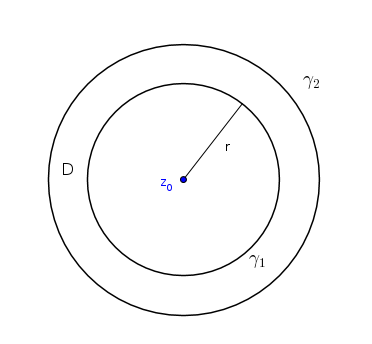
\includegraphics[scale=0.5]{4.png}
\end{center}
$\displaystyle{\sum_{n = 0}^{\infty} a_n (z-z_0)^n}$ es la parte analítica \\
$\displaystyle{\sum_{n = 0}^{\infty} b_n (z-z_0)^n}$ es la parte principal \\
\subsection{TEOREMA.-}
Sea $f(z)$ una función analítica en el anillo $\displaystyle{\gamma_1 < \parallel z - z_0 \parallel < \gamma_2}$, entonces para $z$ en este anillo $\displaystyle{f(z) = \sum_{n = 0}^{\infty} a_n (z-z_0)^n}$ donde $\displaystyle{a_n = \oint_{\gamma_1} \dfrac{f(w) dw}{(w-z_0)^{n+1}}}$ para $\displaystyle{n = 0, +- 1, +-2,...,}$ y $\gamma$ es cualquier circunferencia $\parallel  z - z_0 \parallel = \rho$, con $r_1 < \rho < r_2$\\
 %grafico 335
\begin{center}
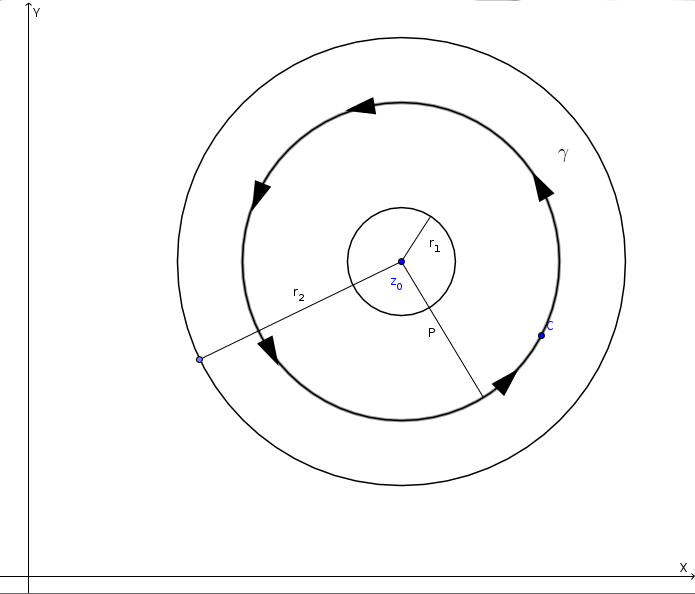
\includegraphics[scale=0.25]{5.png}
\end{center}
 \begin{center}
  \textbf{\underline{Demostración}}
  \end{center} 
Sea $z$ en el anillo, elegimos los números $R_1$ y $R_2$, tal que $\displaystyle{r_1 < R_1 <  \parallel z -z_0  \parallel < R_2 < r_2}$, tal como en la figura: \\
%Grafico 335
\begin{center}
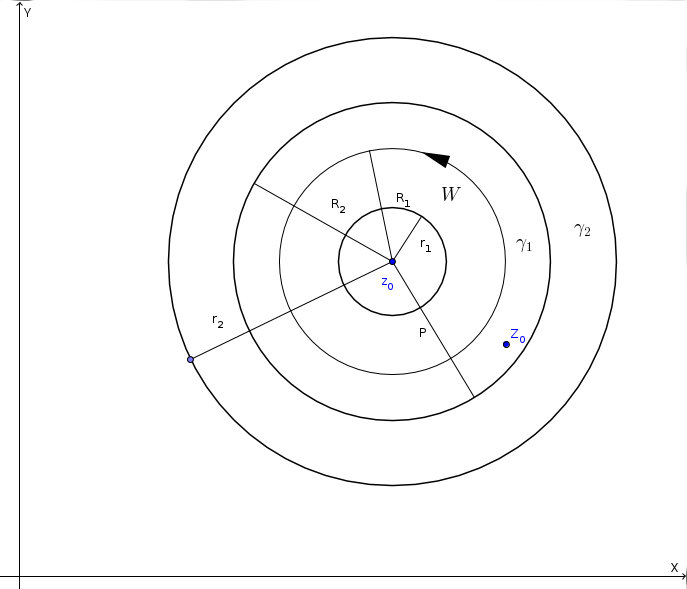
\includegraphics[scale=0.25]{6.png}
\end{center}
Sea $\gamma_2 : \parallel z - z_0 \parallel = R_2$, la circunferencia de radio $R_2$ y $\gamma_1 : \parallel z -z_0 \parallel = R_1$, la circunferencia de radio $R_1$\\
Por la fórmula generalizada del teorema de Integral de Cauchy se puede escribir: \\
$\displaystyle{f(z) = \dfrac{1}{2 \pi i} \oint_{\gamma_2} \dfrac{f(w)dw}{w-z} - \dfrac{1}{2 \pi i} \oint_{\gamma_1} \dfrac{f(w)}{w-z}dz }$		
calculando ambas integrales en el sentido contrario al movimiento de las manecillas del reloj. \\
Consideremos las integrales de línea por separado para la integral $\displaystyle{\dfrac{1}{2 \pi i} \oint_{\gamma_2} \dfrac{f(w)dw}{w-z}}$ escribiremos $\displaystyle{\dfrac{1}{w-z} = \sum_{n=0}^{\infty} \dfrac{(z-z_0)^n}{(w-z_0)^{n+1}}}$, entonces se tiene\\
$\displaystyle{\dfrac{1}{2 \pi i} \oint_{\gamma_2} \dfrac{f(w)dw}{w-z} = \dfrac{1}{2 \pi i} \oint_{\gamma_2} \sum_{n=0}^{\infty}  \dfrac{(z-z_0)^n f(w)}{(w-z_0)^{n+1}} dw =  \sum_{n=0}^{\infty} [ \dfrac{1}{2 \pi i} \oint_{\gamma_2} \dfrac{f(w) dw}{(w-z_0)^{n+1}}] (z-z_0)^n=\sum_{n = 0}^{\infty} a_n (z-z_0)^n}$ , donde $\displaystyle{a_n = \dfrac{1}{2 \pi i} \oint_{\gamma_2} \dfrac{f(w) dw}{(w-z_0)^{n+1}}}$; para $\displaystyle{n = 0,+-1,+-2,...}$ \\
para la integral $\displaystyle{\oint_{\gamma_1} \dfrac{f(w) dw}{w-z}}$, escribiremos en la forma \\
$\displaystyle{\dfrac{1}{w-z} = \dfrac{1}{(w-z_0)-(z-z_0)} = - \dfrac{1}{z-z_0}.\dfrac{1}{1-\dfrac{w-z_0}{z-z_0}}}$, se observa que para $w \epsilon \gamma_1$, se tiene: \\
$\displaystyle{\parallel \dfrac{w-z_0}{z-z_0} \parallel < 1}$, luego por la serie geométrica se tiene: \\
$\displaystyle{\dfrac{1}{w-z} = - \dfrac{1}{z-z_0}.\dfrac{1}{1-\dfrac{w-z_0}{z-z_0}} = -\dfrac{1}{z-z_0} \sum_{n = 0}^{\infty} (\dfrac{w-z_0}{z-z_0})^n = - \sum_{n = 0}^{\infty} \dfrac{(w-z_0)^n}{(z-z_0)^{n+1}} = - \sum_{n = 1}^{\infty} \dfrac{(w-z_0)^{n-1}}{(z-z_0)^{n}} }$, por lo tanto se tiene:\\
$\displaystyle{\dfrac{1}{2 \pi i} \oint_{\gamma_1} \dfrac{f(w)dw}{w-z} = -\sum_{n = 0}^{\infty} [\dfrac{1}{2 \pi i} \oint_{\gamma_1} f(w)(w-z_0)^{n-1}dw] \dfrac{1}{(z-z_0)^n}}$ \\
donde $\displaystyle{a_n = \dfrac{1}{2 \pi i} \oint_{\gamma_1} f(w) (w-z_0)^{n-1}dw }$, para $n = 1,2,3,...$ ahora utilizamos el teorema de la deformación para reemplazar $\gamma_1$ y $\gamma_2$ con la circunferencia $\gamma_\rho : \parallel z - z_0 \parallel = \rho$, esto nos sirve para expresar una fórmula para $a_0,a_1,a_2,...,a_{-1},a_{-2},...,$ en una sola fórmula\\
$\displaystyle{a_n = \dfrac{1}{2 \pi i} \oint_{\gamma_2} \dfrac{f(w)dw}{w-z} - \dfrac{1}{2 \pi i} \oint_{\gamma_1} \dfrac{f(w)dw}{w-z}= \sum_{n=0}^{\infty} a_n (z-z_0)^n + \sum_{n=1}^{\infty} a_{-n} (\dfrac{1}{(z-z_0)^n})}$\\
$\displaystyle{\sum_{n=0}^{\infty} a_n (z-z_0)^n}$\begin{center}
 $\displaystyle{\therefore f(z) = \sum_{n=0}^{\infty} a_n (z-z_0)^n}$
\end{center}
\subsection{EJERCICIOS DESARROLLADOS.-}

\end{document}
